\documentclass[12pt]{article}
\usepackage[utf8]{inputenc}
\usepackage{graphicx}
%\usepackage[margin=0.5in]{geometry}
\usepackage{hyperref}
\title{\Huge{Unbabel Java Challenge}}
\author{Tomasz Szypuła}
\date{\today}

\begin{document}
\maketitle
\section{Project Overview and Objectives }
\paragraph{The goal}of the challenge was to write a Java Application meeting the requieremtns specified in the \href{ https://github.com/Unbabel/java-coding-challenge}{java-coding-challenge}.

 


\section{The Application}
\texttt{java --module-path \$PATH\_TO\_JAVAFX\_DIR/javafx-sdk-11.0.2/lib \\--add-modules=javafx.controls,javafx.fxml \\-jar java-coding-challenge.jar \$USERNAME \$API\_KEY}

\begin{figure}
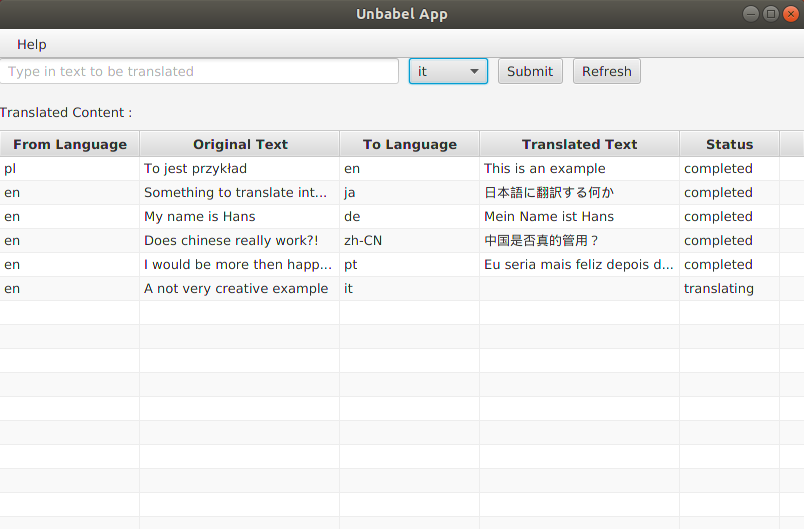
\includegraphics[scale=0.5]{appExample.png}
\end{figure}
\end{document}